% Mothbox Pro, field setup manual (A4 landscape, English)
% Build: pdflatex notice-mothbox-en.tex (two passes)
\documentclass[10pt,a4paper]{article}
\usepackage[T1]{fontenc}
\usepackage[utf8]{inputenc}
\usepackage[english]{babel}
\usepackage[default,semibold]{sourcesanspro}
\usepackage[landscape,top=1.5cm,bottom=1.4cm,left=1.6cm,right=1.6cm,headheight=13pt,headsep=12pt,footskip=20pt]{geometry}
\usepackage{xcolor,graphicx,tabularx,booktabs,array,enumitem,multicol}
\usepackage{fancyhdr,titlesec,tikz,fontawesome5}
\usepackage[hidelinks]{hyperref}
\usetikzlibrary{calc}

\definecolor{marque}{HTML}{2E6B4F}
\definecolor{trait}{HTML}{9A9A9A}
\definecolor{fondgris}{HTML}{F2F2F2}

\graphicspath{{annotees_notice_en/}{annotees_notice/}{photos/}}
\setlength{\parindent}{0pt}
\setlength{\parskip}{4pt}
\setlist{itemsep=2pt,topsep=2pt,leftmargin=1.4em}
\setlist[itemize]{label=\textbullet}
\renewcommand{\arraystretch}{1.25}
\newcolumntype{L}{>{\raggedright\arraybackslash}X}

\pagestyle{fancy}
\fancyhf{}
\fancyhead[L]{\footnotesize Mothbox Pro \textbar{} Field setup manual}
\fancyhead[R]{\footnotesize Ref. MB-NP-01-EN \textbar{} Rev. A}
\fancyfoot[L]{\footnotesize EN}
\fancyfoot[R]{\footnotesize \thepage}
\renewcommand{\headrulewidth}{0.4pt}

\titleformat{\section}{\Large\bfseries}{\textcolor{marque}{\thesection}}{0.6em}{}[\vspace{-6pt}\rule{\linewidth}{0.4pt}]
\titleformat{\subsection}{\normalsize\bfseries}{\thesubsection}{0.6em}{}
\titlespacing*{\section}{0pt}{2pt}{8pt}
\titlespacing*{\subsection}{0pt}{8pt}{2pt}

\newcommand{\sw}[1]{\textbf{#1}}
\newcommand{\rep}[1]{\tikz[baseline=(n.base)]\node[circle,draw,line width=0.6pt,inner sep=0.8pt,minimum size=1.15em,font=\footnotesize\bfseries](n){#1};}

\newcommand{\avert}[2]{%
  \par\smallskip\noindent
  \begin{tabularx}{\linewidth}{@{}p{0.75cm}!{\color{black}\vrule width 1.2pt}@{\hspace{6pt}}X@{}}
  \raisebox{-2pt}{\Large\faExclamationTriangle} & \textbf{#1}\quad #2
  \end{tabularx}\par\smallskip}
\newcommand{\remarque}[1]{%
  \par\smallskip\noindent
  \begin{tabularx}{\linewidth}{@{}p{0.75cm}!{\color{trait}\vrule width 1.2pt}@{\hspace{6pt}}X@{}}
  \raisebox{-2pt}{\Large\faInfoCircle} & \textbf{Note}\quad #1
  \end{tabularx}\par\smallskip}

% DIP switch diagram. #1: number of switches; #2: list name/state (1 = ON)
\newcommand{\dip}[2]{%
\begin{tikzpicture}[x=1.0cm,y=0.34cm,baseline=(current bounding box.center)]
  \fill[black,rounded corners=1.5pt] (0,0) rectangle (#1,2.3);
  \foreach \nom/\etat [count=\i] in {#2} {
    \fill[gray!55] (\i-0.82,0.32) rectangle (\i-0.18,1.98);
    \ifnum\etat=1
      \fill[white] (\i-0.78,0.36) rectangle (\i-0.22,1.08);
    \else
      \fill[white] (\i-0.78,1.22) rectangle (\i-0.22,1.94);
    \fi
    \node[font=\scriptsize\bfseries,anchor=south] at (\i-0.5,2.4) {\nom};
  }
  \node[font=\tiny,anchor=east] at (-0.08,0.72) {ON};
  \node[font=\tiny,anchor=east] at (-0.08,1.58) {OFF};
\end{tikzpicture}}


\begin{document}

% ---------------------------------------------------------------- Cover
\thispagestyle{empty}
\begin{minipage}[t][17.4cm][t]{0.46\textwidth}
\vspace{0pt}
{\small\bfseries DINALab}\par\vspace{1pt}
{\small Digital Naturalism Laboratories}\par\vspace{1.8cm}
{\fontsize{40}{44}\selectfont\bfseries Mothbox Pro}\par\vspace{6pt}
{\LARGE Field setup manual}\par\vspace{14pt}
{\color{marque}\rule{3cm}{3pt}}\par\vspace{14pt}
{\large Setting the time and schedule, and testing\\ the Mothbox from a phone}\par
\vfill
\avert{Important}{Read this manual before first use.}
\vspace{10pt}
{\footnotesize
\begin{tabular}{@{}ll@{}}
Software & 5.2.1-webui \\
Circuit board & Mothbox v5.0.5 \\
Reference & MB-NP-01-EN, revision A \\
Date & November 2026 \\
\end{tabular}}
\end{minipage}\hfill
\begin{minipage}[t][17.4cm][c]{0.48\textwidth}
\centering
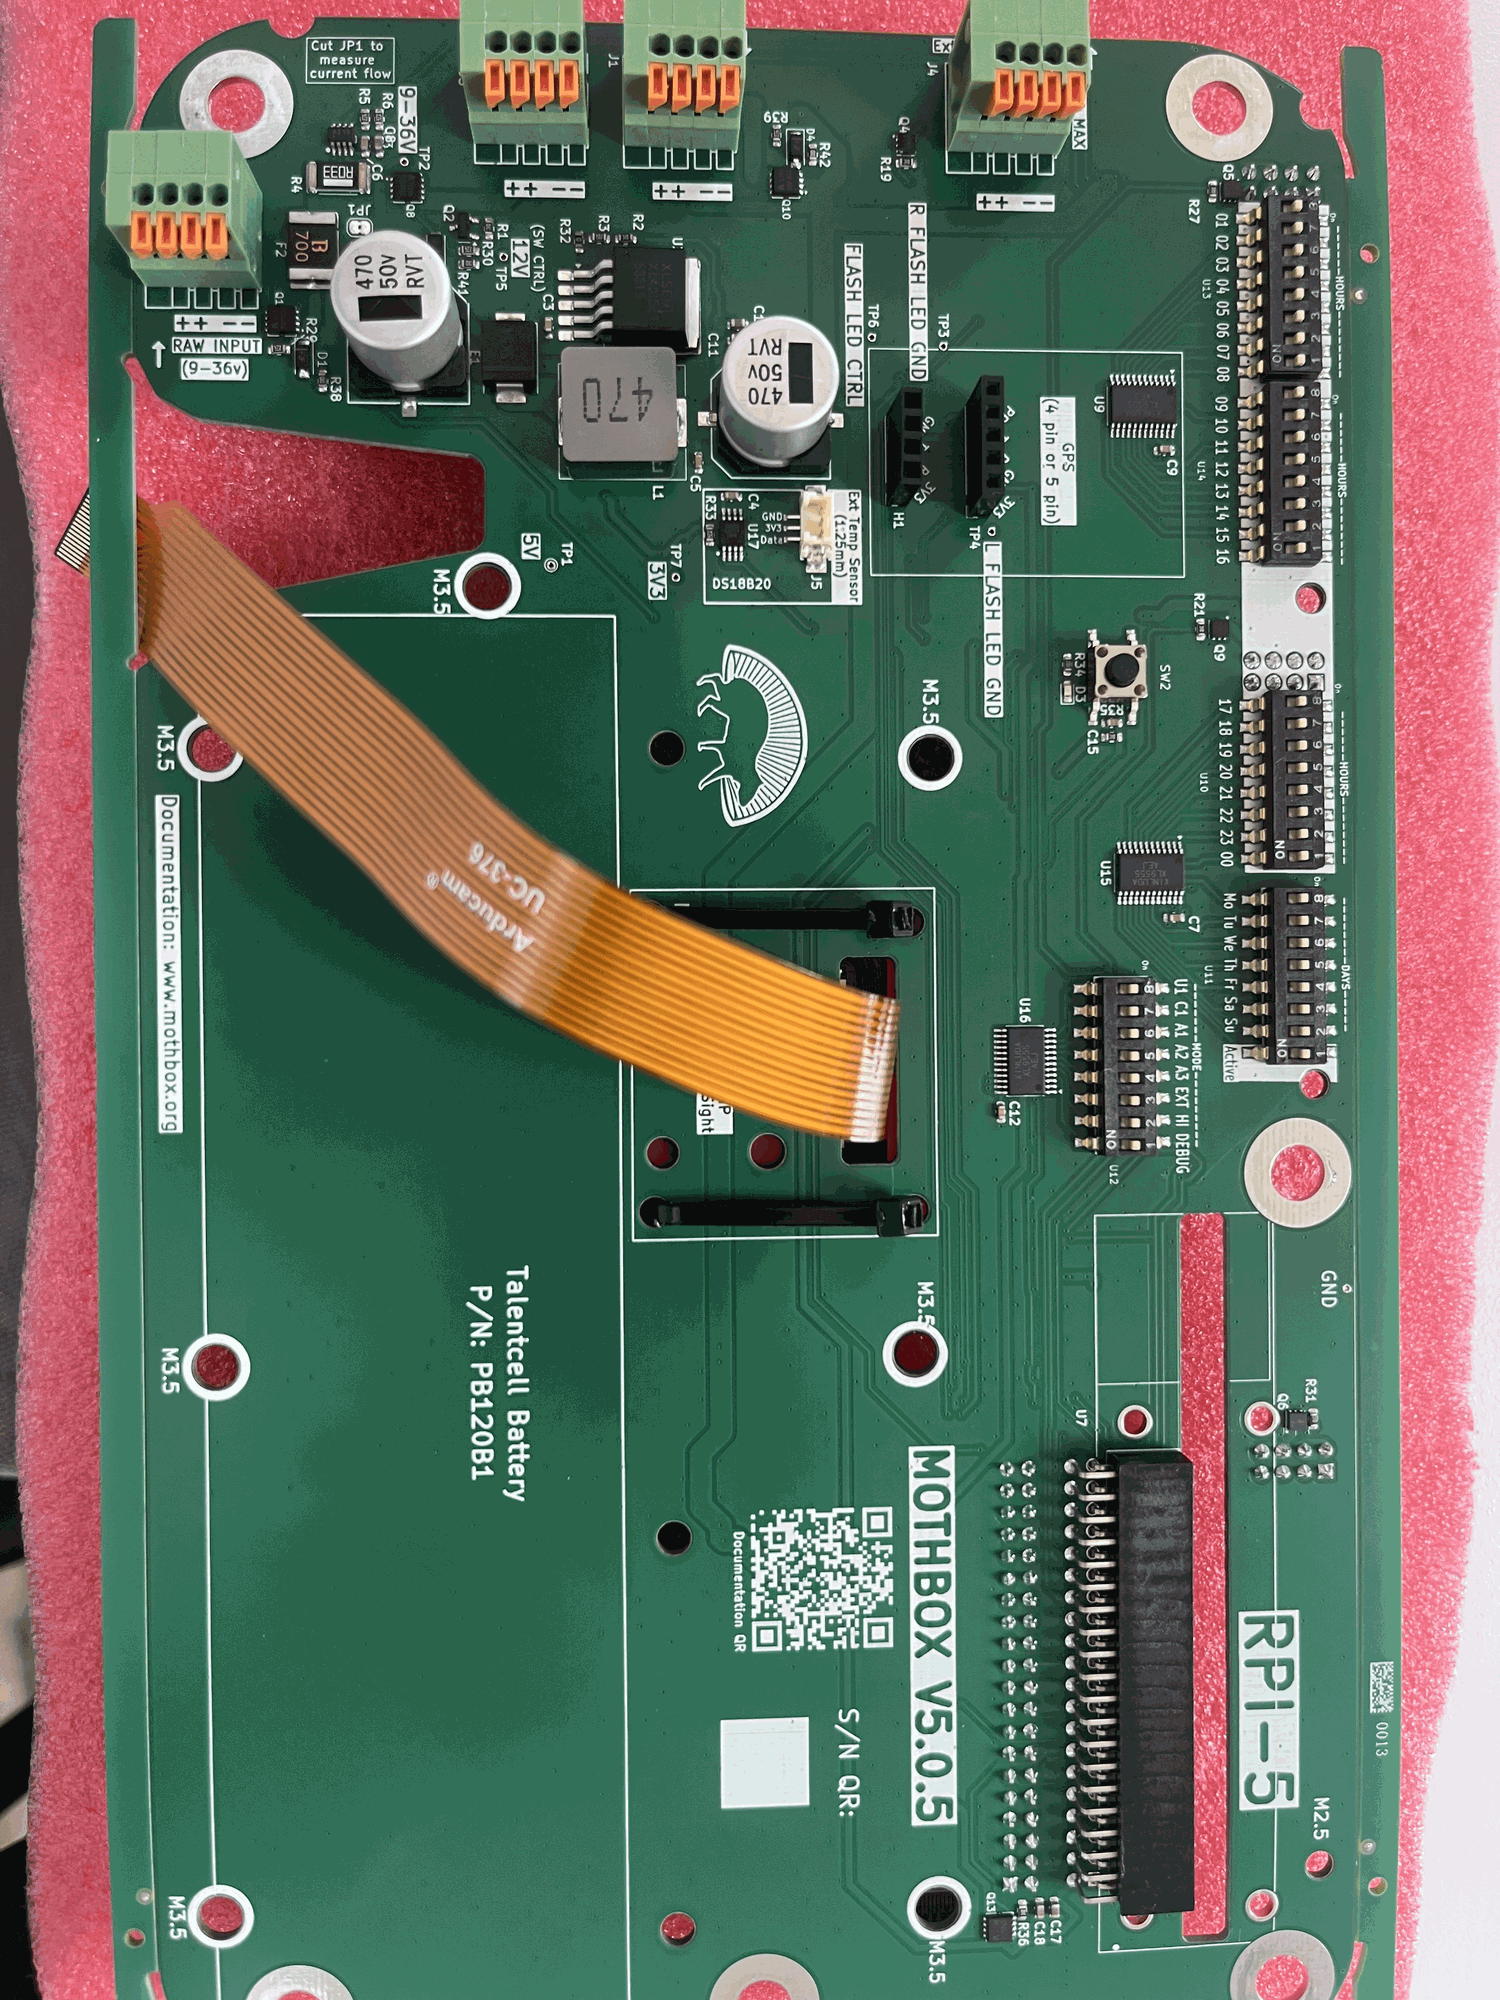
\includegraphics[height=16.8cm,trim=880 120 0 120,clip]{carte_entiere.png}
\end{minipage}

% ---------------------------------------------------------------- Page 2
\newpage
\begin{minipage}[t]{0.40\textwidth}
\vspace{0pt}
\section{Overview}
The Mothbox is set up from a phone or a computer. No app needs to be installed and no Internet connection is required.

When the \sw{DEBUG} switch is ON, the Mothbox creates its own Wi-Fi network and serves a setup page. Once setup is complete, \sw{DEBUG} is set back to OFF and the Mothbox runs on its own, following the chosen schedule.

\subsection{Board layout}
\begin{tabular}{@{}cl@{}}
\rep{1} & Hour switches (01 to 00) \\
\rep{2} & Day switches (Mo to Su) \\
\rep{3} & \sw{Active} switch \\
\rep{4} & \sw{U1} switch, manual mode \\
\rep{5} & MODE row \\
\rep{6} & \sw{DEBUG} switch, setup mode \\
\end{tabular}

\section{Before you start}
You will need:
\begin{itemize}
  \item a Mothbox fitted with an SD card running software 5.2.1-webui;
  \item a charged battery;
  \item a phone or computer with Wi-Fi and a web browser.
\end{itemize}
\avert{Caution}{Switches are read at startup only. Restart the Mothbox after changing any switch.}
\end{minipage}\hfill
\begin{minipage}[t]{0.55\textwidth}
\vspace{0pt}\centering
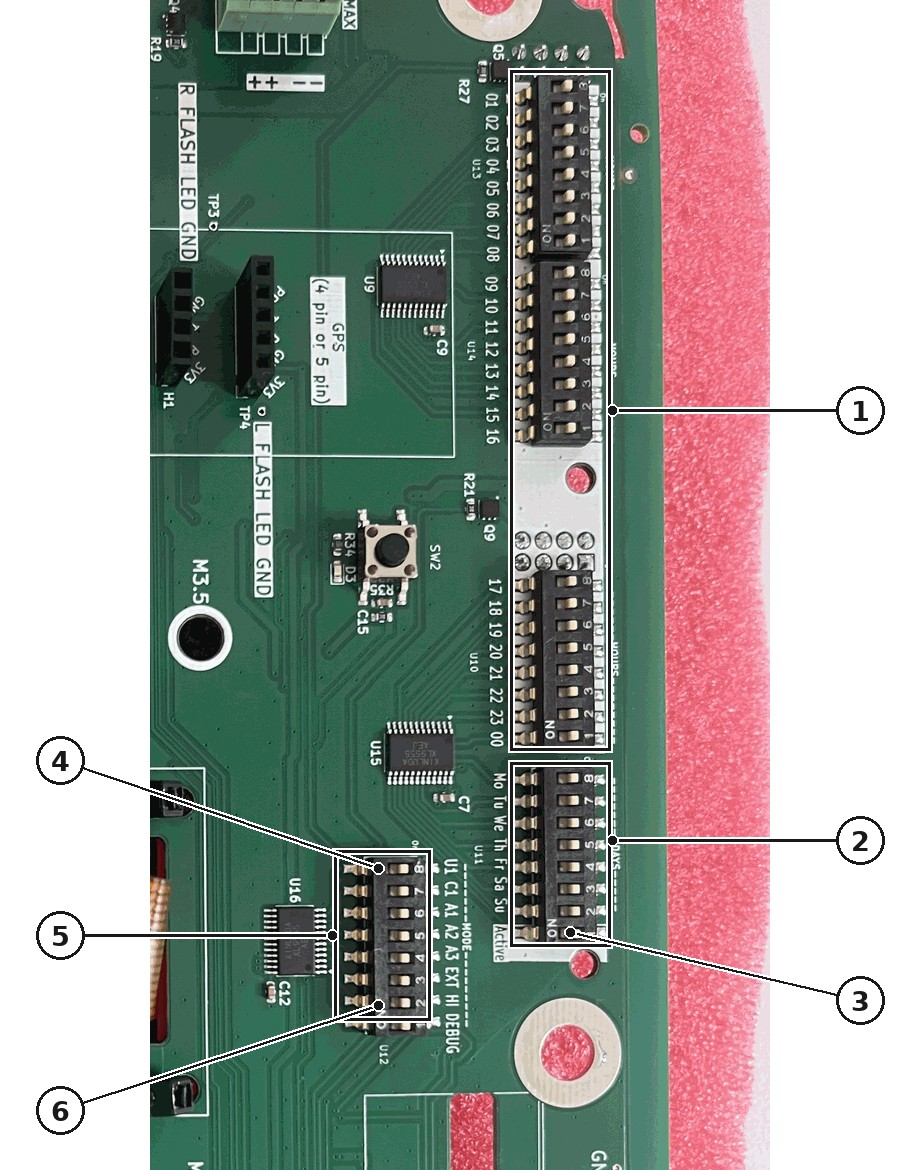
\includegraphics[height=16.6cm]{carte.jpg}\par
{\footnotesize Figure 1: Mothbox v5.0.5 board, switch area}
\end{minipage}

% ---------------------------------------------------------------- Page 3
\newpage
\section{Switches}
\begin{minipage}[t]{0.27\textwidth}
\vspace{0pt}
\subsection{Reading a switch}
A switch is ON when its lever is pushed towards the ON marking on the black switch body, which means downwards on the board.

\begin{center}\dip{1}{/1}\qquad\dip{1}{/0}\\[2pt]
{\footnotesize ON \hspace{1.6cm} OFF}\end{center}

\avert{Caution}{The ``On'' marking printed on the green board, above the switch blocks, does not indicate the ON direction.}
\end{minipage}\hfill
\begin{minipage}[t]{0.69\textwidth}
\vspace{0pt}
\subsection{Operating modes}
\begin{tabularx}{\linewidth}{@{}>{\centering\arraybackslash}m{2.9cm}>{\raggedright\arraybackslash}m{3.4cm}>{\raggedright\arraybackslash}m{9.6cm}}
\toprule
Position & Mode & Mothbox behaviour \\
\midrule
\dip{2}{Active/0,DEBUG/0} & Off \newline storage, transport, charging & Shuts down as soon as it wakes up. \\
\addlinespace[5pt]\dip{2}{Active/1,DEBUG/1} & Setup & Stays on, creates its Wi-Fi network and serves the setup page. No captures. \\
\addlinespace[5pt]\dip{2}{Active/1,DEBUG/0} & Operation & Sleeps, then wakes up at the scheduled times to attract and photograph insects. \\
\addlinespace[5pt]\dip{2}{Active/0,DEBUG/1} & Incorrect position & \sw{Active} takes priority: the Mothbox shuts down and no Wi-Fi network is created. \\
\bottomrule
\end{tabularx}
\end{minipage}

\vspace{6pt}
\subsection{MODE row}
\begin{minipage}[t]{0.33\textwidth}
\vspace{0pt}
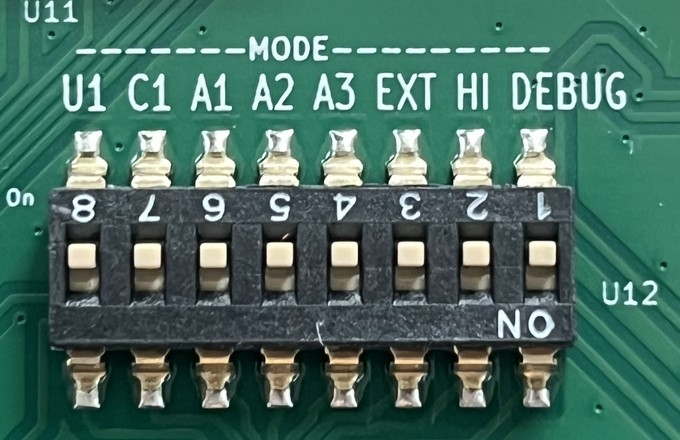
\includegraphics[width=\linewidth]{rangee_mode.jpg}\par
{\footnotesize Figure 2: MODE row, all switches OFF}
\end{minipage}\hfill
\begin{minipage}[t]{0.63\textwidth}
\vspace{0pt}\small
\begin{tabularx}{\linewidth}{@{}>{\bfseries}p{1.9cm}L>{\raggedright\arraybackslash}p{2.6cm}@{}}
\toprule
\normalfont Switch & Function & Recommended position \\
\midrule
U1 & Manual mode: schedule set with the hour and day switches (see section 5). & OFF \\
C1 & Light test, with \sw{DEBUG} ON: the lighting channels and the flash turn on one after another, in a loop. Stopped by restarting. & OFF \\
A1, A2, A3 & Reserved (attraction channel selection). No effect with software 5.2.1. & OFF \\
EXT & Reserved (external attraction output). No effect with software 5.2.1. & OFF \\
HI & Reserved (mains power supply). No effect with software 5.2.1. & OFF \\
DEBUG & Setup mode: Wi-Fi network and setup page. & ON for setup, OFF in operation \\
\bottomrule
\end{tabularx}
\end{minipage}

% ---------------------------------------------------------------- Page 4
\newpage
\section{Setup with a phone}
\begin{minipage}[t]{0.37\textwidth}
\vspace{0pt}
\subsection{Connecting}
\begin{enumerate}
  \item Set \sw{Active} and \sw{DEBUG} to ON.
  \item Connect the battery.
  \item Wait 2 to 3 minutes.
  \item In the phone's Wi-Fi settings, select the \texttt{Mothbox-}\textit{name} network.\\Password: \texttt{lunaluna}.
  \item The setup page opens automatically. If it does not, enter \texttt{192.168.50.5} in the browser.
\end{enumerate}
\remarque{The phone may report that the network has no Internet access. Choose to stay connected to it.}
The page language follows the phone's language. Use the FR/EN button at the top right to change it.

The page has four steps, reached with tabs 1 to 4 or with the \emph{Next step} button.
\end{minipage}\hfill
\begin{minipage}[t]{0.28\textwidth}
\vspace{0pt}\centering
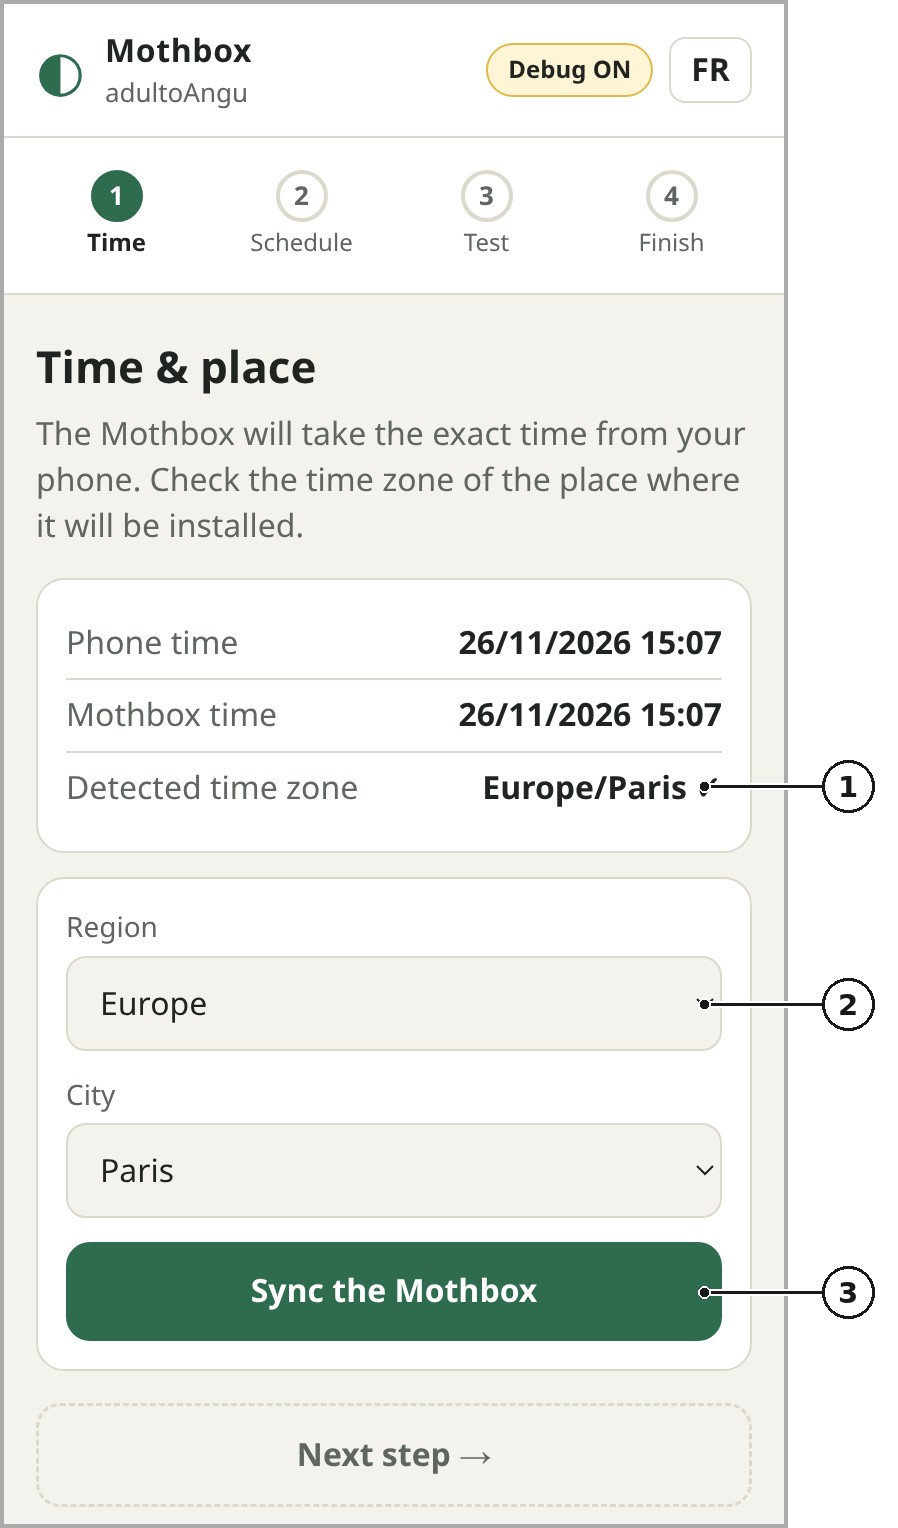
\includegraphics[width=\linewidth]{ecran1.jpg}\par
{\footnotesize Figure 3: step 1, time and place}
\end{minipage}\hfill
\begin{minipage}[t]{0.29\textwidth}
\vspace{0pt}
\subsection{Step 1: time and place}
The Mothbox takes its time from the phone.
\begin{enumerate}
  \item Check the detected time zone \rep{1}.
  \item If the installation site is in another time zone, select the region and city \rep{2}.
  \item Press \emph{Sync the Mothbox} \rep{3}. The corrected offset is displayed.
\end{enumerate}
\remarque{If no time zone is detected, the button stays disabled until a city is selected.}
\end{minipage}

% ---------------------------------------------------------------- Page 5
\newpage
\begin{minipage}[t]{0.25\textwidth}
\vspace{0pt}\centering
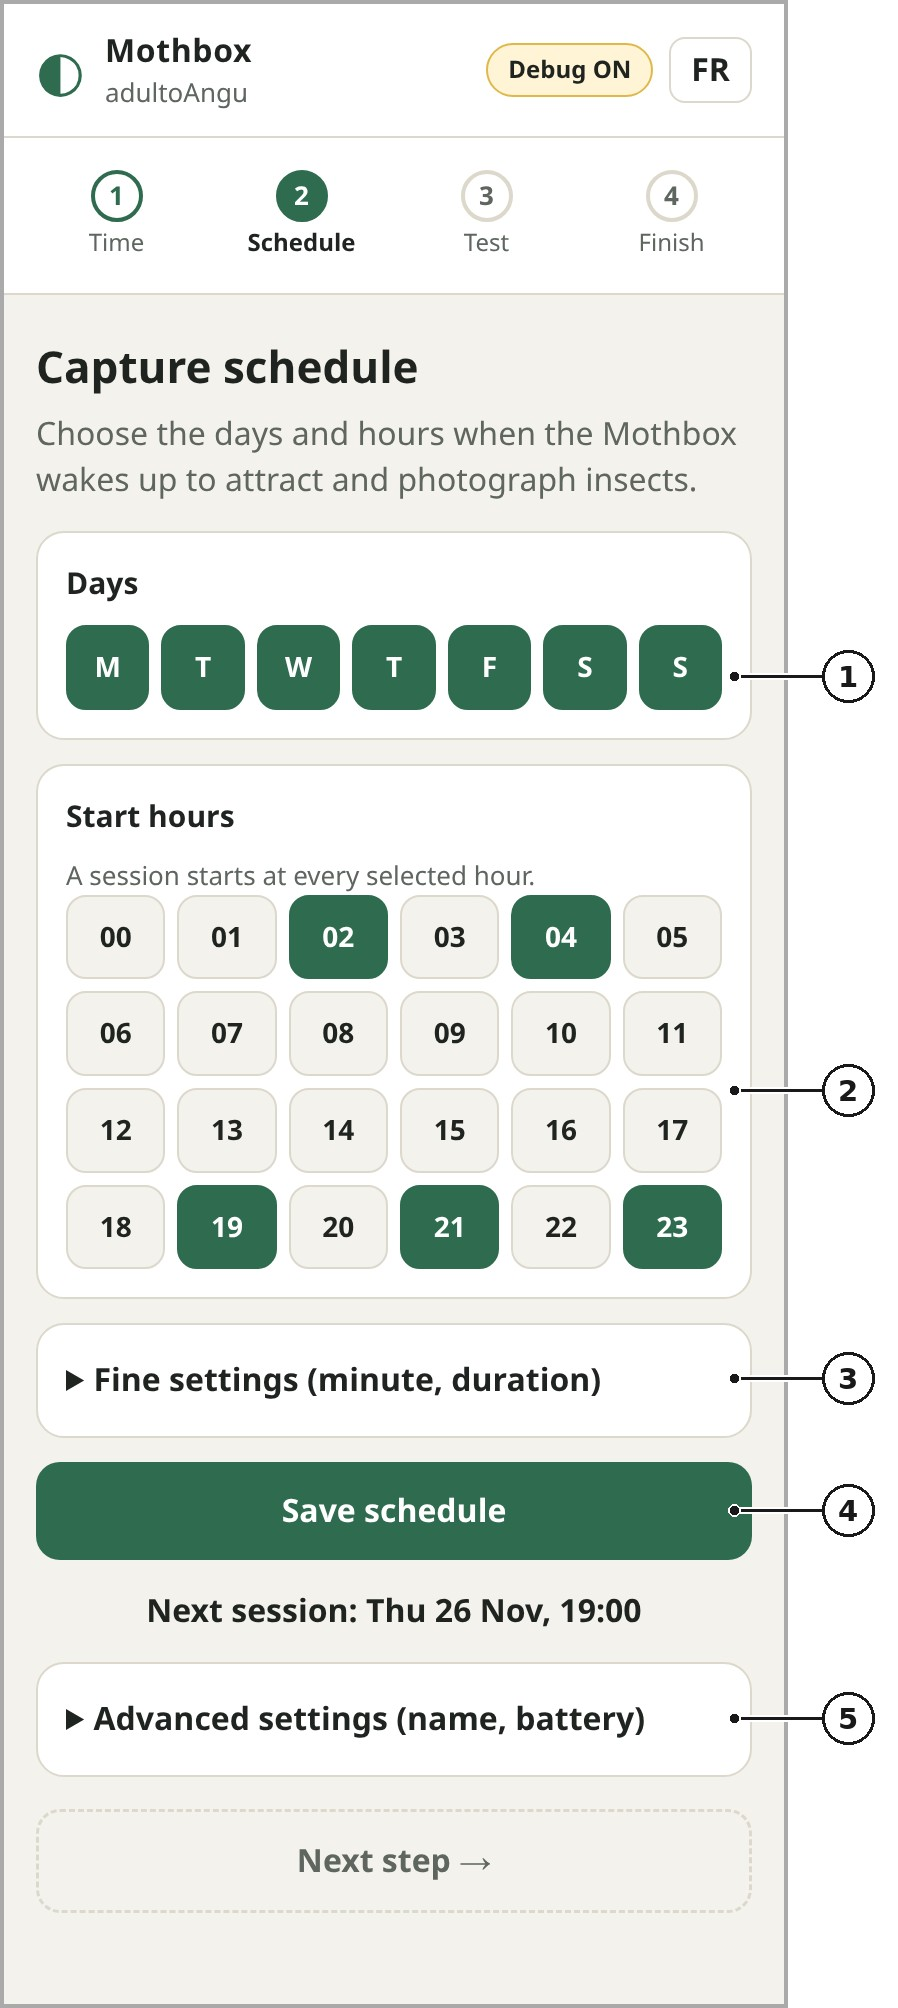
\includegraphics[width=\linewidth]{ecran2.jpg}\par
{\footnotesize Figure 4: step 2, schedule}
\end{minipage}\hfill
\begin{minipage}[t]{0.23\textwidth}
\vspace{0pt}
\subsection*{Step 2: schedule}
\begin{enumerate}
  \item Select the capture days \rep{1}.
  \item Select the start hours \rep{2}. A session starts at every selected hour.
  \item If needed, set the start minute and the session length \rep{3} (59 min by default).
  \item Press \emph{Save schedule} \rep{4}. The next session is displayed.
\end{enumerate}
\emph{Advanced settings} \rep{5} let you change the Mothbox name and the battery characteristics.
\end{minipage}\hfill
\begin{minipage}[t]{0.25\textwidth}
\vspace{0pt}\centering
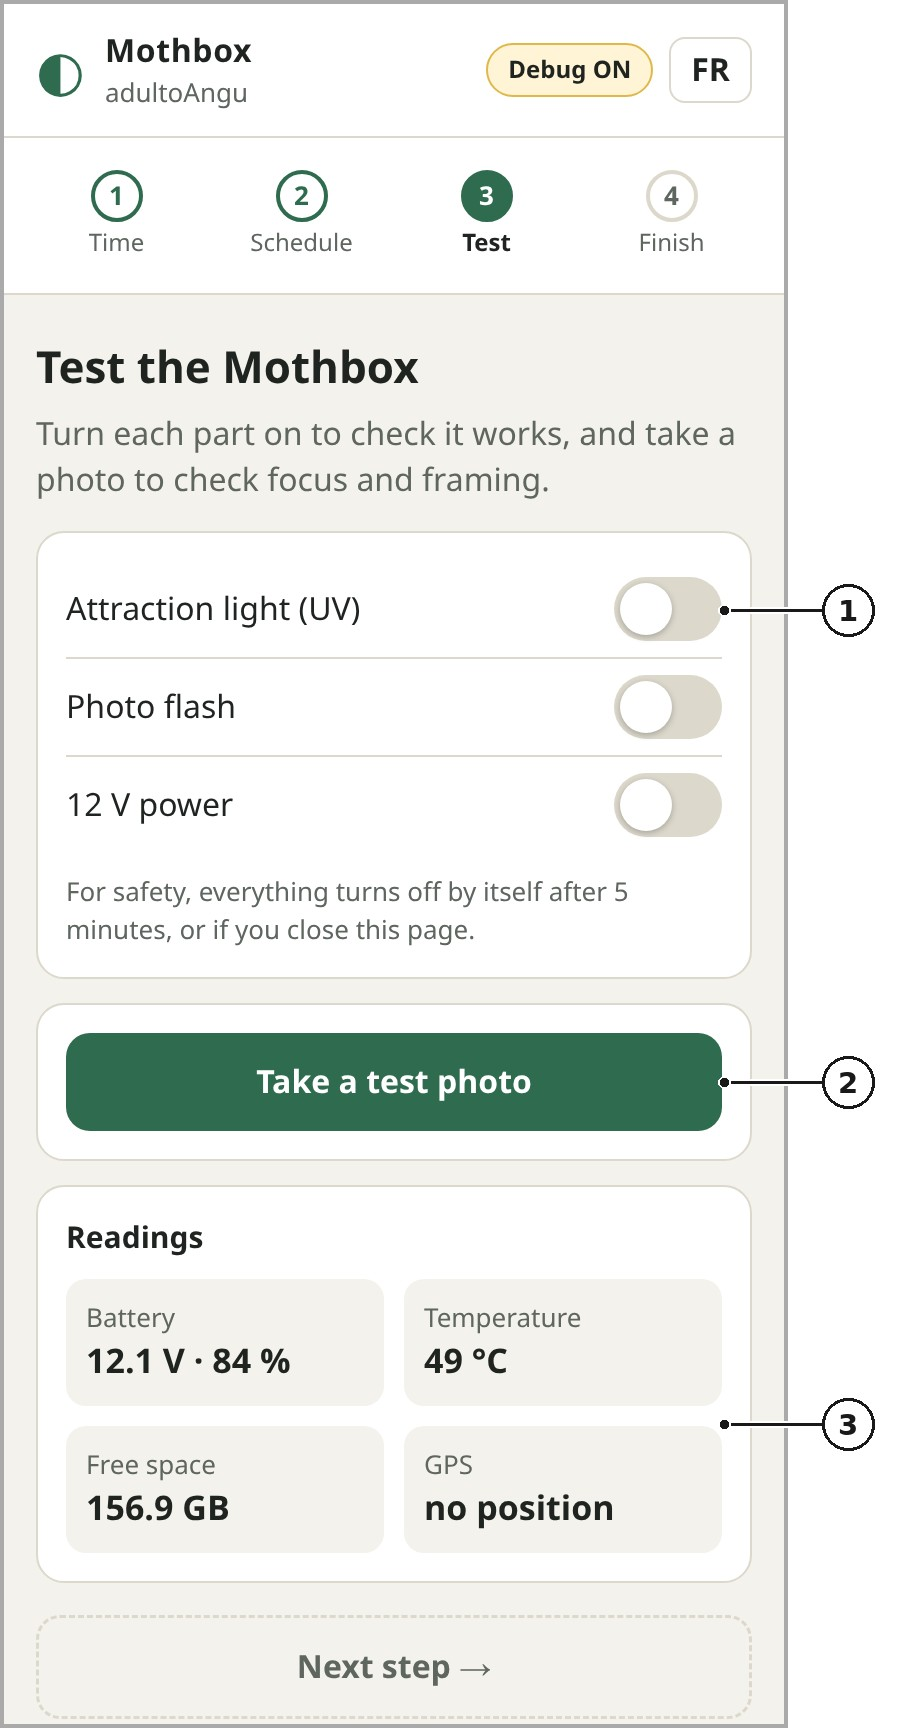
\includegraphics[width=\linewidth]{ecran3.jpg}\par
{\footnotesize Figure 5: step 3, tests}
\end{minipage}\hfill
\begin{minipage}[t]{0.23\textwidth}
\vspace{0pt}
\subsection*{Step 3: tests}
\begin{enumerate}
  \item Turn the attraction light, the flash and the 12\,V power on, then off \rep{1}.
  \item Press \emph{Take a test photo} \rep{2}. Check that the sheet is sharp and fills the frame.
  \item Check the readings \rep{3}: battery, temperature, free space, GPS position.
\end{enumerate}
\remarque{Outputs turn off automatically after 5 minutes, or 30 seconds after the page is closed.}
\end{minipage}

% ---------------------------------------------------------------- Page 6
\newpage
\begin{minipage}[t]{0.22\textwidth}
\vspace{0pt}\centering
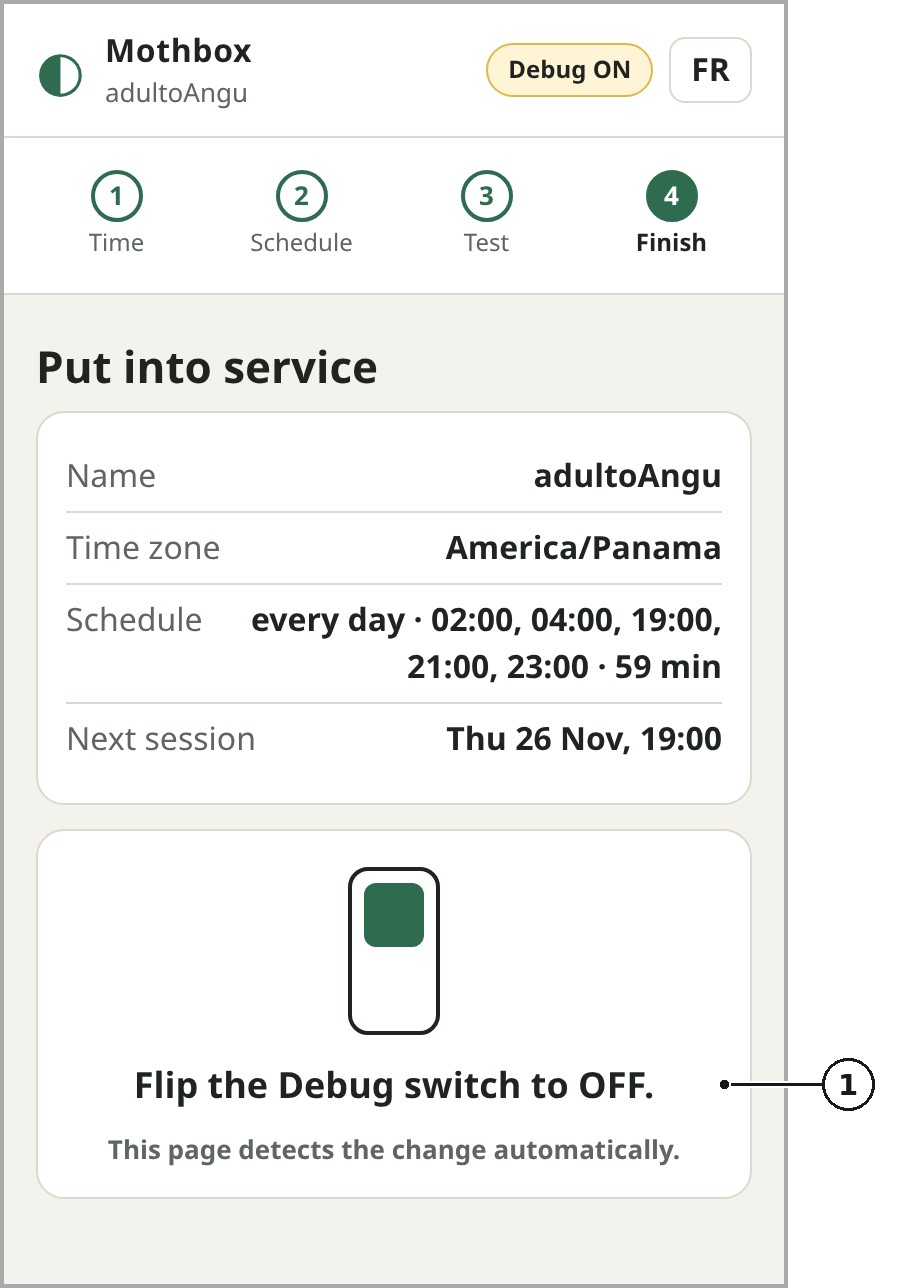
\includegraphics[width=\linewidth]{ecran4.jpg}\par\vspace{4pt}
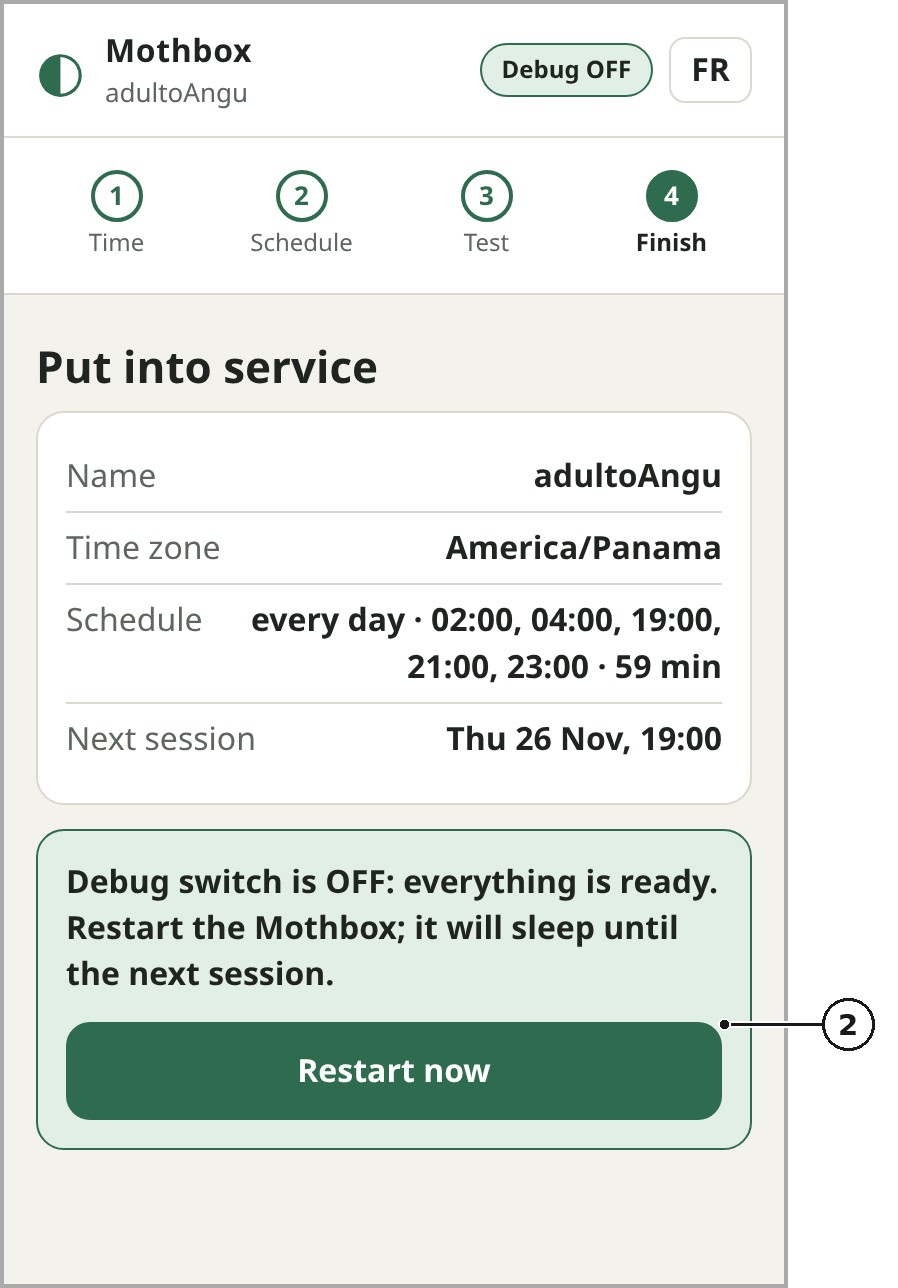
\includegraphics[width=\linewidth]{ecran4_pret.jpg}\par
{\footnotesize Figure 6: step 4, putting into service}
\end{minipage}\hfill
\begin{minipage}[t]{0.33\textwidth}
\vspace{0pt}
\subsection*{Step 4: putting into service}
The page summarises the name, time zone, schedule and next session.
\begin{enumerate}
  \item Set \sw{DEBUG} to OFF \rep{1} without disconnecting the battery. Leave \sw{Active} ON.
  \item Wait for the page to detect the change, then press \emph{Restart now} \rep{2}.
\end{enumerate}
The Mothbox restarts, turns off its Wi-Fi network and sleeps until the next session. The page can be closed.
\avert{Caution}{If the page reports that the Active switch is OFF, set it back to ON. In that position, the Mothbox would shut down every time it wakes up, without taking any photos.}
\end{minipage}\hfill
\begin{minipage}[t]{0.40\textwidth}
\vspace{0pt}
\section{Manual mode}
The schedule can be set directly on the board, without a phone.
\begin{enumerate}
  \item Set \sw{U1} to ON.
  \item Set the switches for the required start hours and days to ON.
  \item Set \sw{Active} to ON and \sw{DEBUG} to OFF.
  \item Restart the Mothbox.
\end{enumerate}
In manual mode, each session starts on the hour and lasts 59 minutes. If no hour is selected, the Mothbox uses 7\,pm, 9\,pm, 11\,pm, 2\,am and 4\,am; if no day is selected, it runs every day.

\begin{minipage}[t]{0.42\linewidth}
\vspace{0pt}
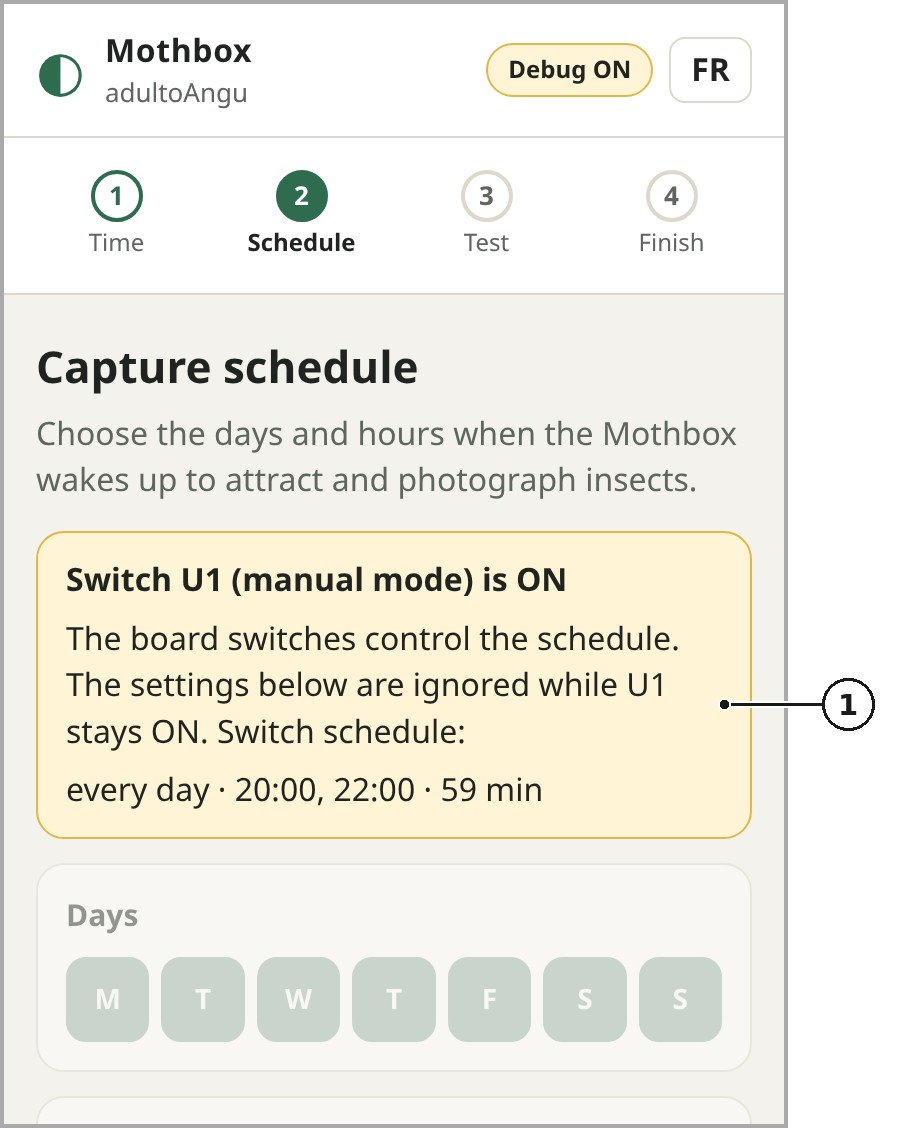
\includegraphics[width=\linewidth]{ecran2_u1.jpg}
\end{minipage}\hfill
\begin{minipage}[t]{0.54\linewidth}
\vspace{0pt}\small
While \sw{U1} is ON, the setup page shows a banner \rep{1} and the schedule read from the switches. The schedule settings on the page are then ignored.
\end{minipage}
\end{minipage}

% ---------------------------------------------------------------- Page 7
\newpage
\section{Troubleshooting}
\small
\begin{tabularx}{\linewidth}{@{}>{\raggedright\arraybackslash}p{5.2cm}>{\raggedright\arraybackslash}p{6.6cm}L@{}}
\toprule
\normalsize\bfseries Problem & \normalsize\bfseries Possible cause & \normalsize\bfseries Solution \\
\midrule
No \texttt{Mothbox-}\textit{name} network & Still starting up. & Wait 3 minutes. \\
 & \sw{Active} or \sw{DEBUG} is OFF. & Set both to ON, then restart. \\
 & Default network name. & Look for the \texttt{mothboxwifi} network. \\
\midrule
Connected, but the page does not open & Automatic opening blocked by the phone. & Enter \texttt{192.168.50.5} in the browser. \\
\midrule
The phone disconnects & The phone is looking for a network with Internet access. & Choose to stay connected; temporarily turn off mobile data. \\
\midrule
``The board did not respond'' message & Light or flash not connected properly. & Check the cables on the terminal blocks, then try again. \\
\midrule
``The camera did not respond'' message & Camera ribbon cable not seated properly. & Check the ribbon cable at both ends, then try again. \\
\midrule
The page keeps waiting for DEBUG to be OFF & Wrong switch flipped. & Flip the last switch of the MODE row, marked DEBUG. \\
\midrule
Captures at the wrong times & Incorrect time zone. & Repeat step 1. \\
 & \sw{U1} is ON. & Set \sw{U1} to OFF if the schedule was set on the page. \\
\midrule
No captures & \sw{Active} is OFF or \sw{DEBUG} is ON. & Set \sw{Active} to ON and \sw{DEBUG} to OFF, then restart. \\
\bottomrule
\end{tabularx}

% ---------------------------------------------------------------- Page 8
\newpage
\begin{minipage}[t]{0.52\textwidth}
\vspace{0pt}
\section{Preparing an SD card}
Use the free Raspberry Pi Imager software (Windows, macOS, Linux), available from \texttt{raspberrypi.com/software}.

File to use: \texttt{mothbox\_Pro\_Pi5\_v5.2.1-webui\_2026-11-26.zip}. Do not unzip it.
\begin{enumerate}
  \item Insert an SD card of at least 16\,GB into the computer.
  \item In Raspberry Pi Imager, choose the \emph{Raspberry Pi 5} device.
  \item Under \emph{Operating System}, choose \emph{Use custom} (at the bottom of the list), then select the file.
  \item Under \emph{Storage}, select the SD card.
  \item When asked about OS customisation, answer \emph{No}.
  \item Wait until writing and verification are complete (about 10 minutes), then remove the card.
\end{enumerate}
\avert{Caution}{All data on the SD card is erased. Check the size of the selected drive before writing.}
\avert{Caution}{Do not customise the OS (user name, password, Wi-Fi): the Mothbox might no longer create its own network.}
\end{minipage}\hfill
\begin{minipage}[t]{0.43\textwidth}
\vspace{0pt}
\section{Specifications}
\small
\begin{tabularx}{\linewidth}{@{}>{\raggedright\arraybackslash}p{4.2cm}L@{}}
\toprule
Software & 5.2.1-webui, based on Mothbox 5.2.1 \\
Compatible hardware & Mothbox Pro, board v5.0.x, Raspberry Pi 5 \\
\midrule
Wi-Fi network (setup mode) & \texttt{Mothbox-}\textit{name} \\
Password & \texttt{lunaluna} \\
Page address & \texttt{192.168.50.5} \\
Languages & French, English \\
\midrule
Programmable days & Monday to Sunday \\
Start hours & 00:00 to 23:00, several per day \\
Session length & 1 to 1439 minutes (59 by default) \\
Manual mode schedule & on the hour, 59 minutes \\
\midrule
Automatic output shutdown & 5 minutes after switching on \\
 & 30 seconds after the page is closed \\
Clock & kept when powered off (RTC battery) \\
\bottomrule
\end{tabularx}
\end{minipage}

\end{document}
